\documentclass[11pt,a4paper]{article}

\usepackage[margin=2.3cm]{geometry}
\usepackage{amsmath,amssymb,amsthm,mathtools}
\usepackage{booktabs,tabularx,array,multirow}
\usepackage{graphicx}
\usepackage[dvipsnames]{xcolor}
\usepackage{tikz}
\usetikzlibrary{arrows.meta,positioning,calc,fit,backgrounds,decorations.pathreplacing}
\usepackage{algorithm}
\usepackage[noend]{algpseudocode}
\usepackage{float}
\usepackage{rotating}
\usepackage{enumitem}
\usepackage[font=small,labelfont=bf]{caption}
\usepackage{microtype}
\usepackage[colorlinks=true,linkcolor=NavyBlue,urlcolor=NavyBlue,citecolor=NavyBlue]{hyperref}
\usepackage[nameinlink,capitalise]{cleveref}
\makeatletter\def\theHALG@line{\thealgorithm.\arabic{ALG@line}}\makeatother

\definecolor{cblue}{HTML}{2A78D6}
\definecolor{corange}{HTML}{EB6834}
\definecolor{cgreen}{HTML}{1BAF7A}
\definecolor{clate}{HTML}{EC835A}
\definecolor{cgrey}{HTML}{E1E0D9}
\definecolor{cink}{HTML}{52514E}

\theoremstyle{plain}
\newtheorem{proposition}{Proposition}
\newtheorem{theorem}[proposition]{Theorem}
\newtheorem{lemma}[proposition]{Lemma}
\theoremstyle{definition}
\newtheorem{definition}{Definition}
\theoremstyle{remark}
\newtheorem*{remark}{Remark}

\newcommand{\Hor}{\mathcal{H}}
\newcommand{\Q}{\mathcal{Q}}
\newcommand{\Sset}{\mathcal{S}}
\newcommand{\J}{\mathcal{J}}
\newcommand{\Leg}{\mathcal{L}}
\newcommand{\QS}[1]{\mathcal{Q}^{S}_{#1}}
\newcommand{\QJ}[1]{\mathcal{Q}^{J}_{#1}}
\newcommand{\V}[1]{\mathcal{V}_{#1}}
\newcommand{\avail}[1]{\alpha_{#1}}
\newcommand{\eqtag}[1]{\tag{#1}}

\setlist{itemsep=2pt,topsep=4pt}
\setlength{\parskip}{3pt}

\title{\textbf{CompuOpti: multi-objective staff scheduling}\\[4pt]
\large Model, equations and exact Pareto methods}
\author{Decision Modelling project (V.~Mousseau), CentraleSup\'elec}
\date{November 2026}

\begin{document}
\maketitle

\begin{abstract}
\noindent
CompuOpti must decide which employee works on which project, with which skill, on which day, over a
horizon of working days. The three given instances ask for more person-days than the staff can
supply, so the real decision is which projects to accept. We formulate the problem as a 0/1 model
solved with Google OR-Tools CP-SAT, using a \emph{time-window} encoding that measures project
duration and lateness without big-$M$ constants. We optimise the brief's four objectives (profit,
longest project, projects per employee, late projects) and two of our own (largest team, fairness
gap). Two exact methods compute the non-dominated set: an $\varepsilon$-constraint method for two
objectives and a disjunctive exclusion method for any number. A separate certificate based on Hall's
theorem proves the maximum profit independently of the solver. This document states every set,
variable, constraint and objective, and proves why each method is exact.
\end{abstract}

\tableofcontents
\vspace{1em}
\hrule

%=====================================================================
\section{The problem}
%=====================================================================

The horizon is a set of working days. Each employee has qualifications (skills) and holiday days.
Each project needs a given number of person-days in each of its skills, brings a gain if delivered,
and pays a daily penalty for every day it finishes after its due date. A schedule assigns every
employee-day either to one (project, skill) pair or to nothing. The brief imposes five hard rules:

\begin{enumerate}[label=\textbf{R\arabic*}]
  \item \textbf{Qualification:} an employee only works with a skill they hold.
  \item \textbf{Uniqueness per day:} one project and one skill per employee per day.
  \item \textbf{Leave:} nobody works on a holiday.
  \item \textbf{Coverage:} a project counts as done only if every required person-day is covered.
  \item \textbf{At most once:} each project is executed at most once in the horizon.
\end{enumerate}

\Cref{fig:pipeline} shows the whole method; the rest of this document details each box.

\begin{figure}[ht]
\centering
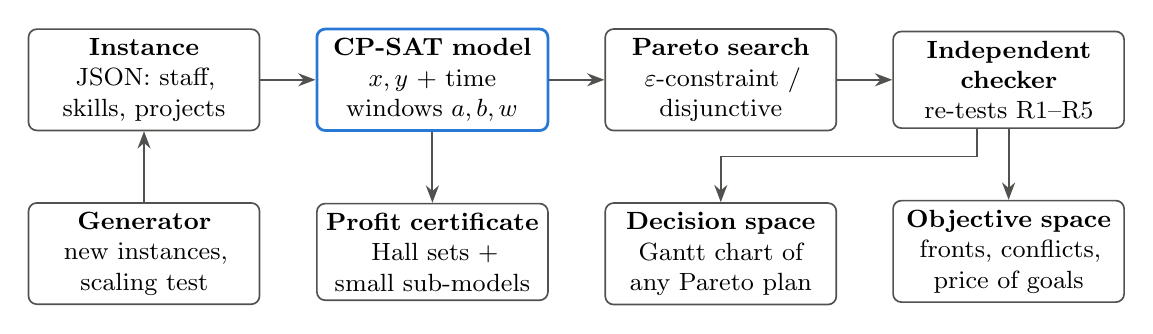
\begin{tikzpicture}[
  node distance=5mm and 7mm,
  box/.style={draw=cink, rounded corners=3pt, fill=white, align=center, font=\small,
              minimum height=11mm, text width=27mm, line width=0.6pt},
  hl/.style={box, draw=cblue, line width=1pt},
  arr/.style={-{Stealth[length=2.2mm]}, cink, line width=0.7pt}]
  \node[box] (data) {\textbf{Instance}\\ JSON: staff,\\ skills, projects};
  \node[hl, right=of data] (model) {\textbf{CP-SAT model}\\ $x,y$ + time\\ windows $a,b,w$};
  \node[box, right=of model] (pareto) {\textbf{Pareto search}\\ $\varepsilon$-constraint /\\ disjunctive};
  \node[box, right=of pareto] (check) {\textbf{Independent}\\ \textbf{checker}\\ re-tests R1--R5};
  \node[box, below=9mm of model] (cert) {\textbf{Profit certificate}\\ Hall sets +\\ small sub-models};
  \node[box, below=9mm of check] (viz) {\textbf{Objective space}\\ fronts, conflicts,\\ price of goals};
  \node[box, below=9mm of pareto] (dec) {\textbf{Decision space}\\ Gantt chart of\\ any Pareto plan};
  \node[box, below=9mm of data] (gen) {\textbf{Generator}\\ new instances,\\ scaling test};
  \draw[arr] (data) -- (model);
  \draw[arr] (model) -- (pareto);
  \draw[arr] (pareto) -- (check);
  \draw[arr] (model) -- (cert);
  \draw[arr] (check) -- (viz);
  \draw[arr] (check.south) ++(-4mm,0) |- ++(0,-3.5mm) -| (dec.north);
  \draw[arr] (gen) -- (data);
\end{tikzpicture}
\caption{Pipeline. Every number we report goes through the independent checker, never straight
from the solver.}
\label{fig:pipeline}
\end{figure}

%=====================================================================
\section{Notation}
%=====================================================================

We keep the notation of the course's reference model and add the symbols our formulation needs.

\begin{table}[H]
\centering\small
\begin{tabularx}{\linewidth}{@{}l X@{}}
\toprule
\textbf{Symbol} & \textbf{Meaning} \\
\midrule
$\Hor=\{1,\dots,h\}$ & working days of the horizon \\
$\Q$ & set of qualifications (skills) \\
$\Sset$ & set of employees; $\QS{i}\subseteq\Q$ skills of $i$; $\V{i}\subseteq\Hor$ holidays of $i$ \\
$\avail{i}=|\Hor\setminus\V{i}|$ & number of days employee $i$ can work \\
$\J$ & set of projects; $\QJ{j}\subseteq\Q$ skills needed by project $j$ \\
$n_{j,k}\in\mathbb{N}$ & person-days of skill $k\in\QJ{j}$ needed by project $j$ \\
$g_j,\ c_j,\ d_j$ & gain, daily late penalty and due date of project $j$ \\
$\Leg$ & \emph{legal slots}: $\{(i,j,k,t) : k\in\QS{i}\cap\QJ{j},\ t\in\Hor\setminus\V{i}\}$ \\
$\Sset_k=\{i: k\in\QS{i}\}$ & holders of skill $k$ \\
\bottomrule
\end{tabularx}
\caption{Sets and parameters (fixed data).}
\label{tab:notation}
\end{table}

%=====================================================================
\section{Decision variables}
%=====================================================================

The central variable is $x$; the others are derived from it and only exist to express the
objectives linearly.

\begin{table}[H]
\centering\small
\begin{tabularx}{\linewidth}{@{}l l X@{}}
\toprule
\textbf{Variable} & \textbf{Domain} & \textbf{Interpretation} \\
\midrule
$x_{i,j,k,t}$ & $\{0,1\}$, $(i,j,k,t)\in\Leg$ & employee $i$ works on skill $k$ of project $j$ on day $t$ \\
$y_j$ & $\{0,1\}$, $j\in\J$ & project $j$ is delivered \\
$a_{j,t}$ & $\{0,1\}$, $j\in\J,t\in\Hor$ & project $j$ has \emph{started} by day $t$ \\
$b_{j,t}$ & $\{0,1\}$, $j\in\J,t\in\Hor$ & project $j$ is \emph{still open} on day $t$ \\
$w_{j,t}$ & $\{0,1\}$, $j\in\J,t\in\Hor$ & day $t$ is inside the \emph{window} of project $j$ ($w=a\wedge b$) \\
$u_{i,j}$ & $\{0,1\}$ & employee $i$ works on project $j$ at least once \\
$v_1,\dots,v_6$ & $\mathbb{Z}$, bounded & one variable per objective (\cref{sec:objectives}) \\
\bottomrule
\end{tabularx}
\caption{Decision variables. $x$ is only created on legal slots, so rules R1 and R3 hold by
construction and the model stays small (3{,}939 $x$-variables on the large instance instead of
$|\Sset|\,|\J|\,|\Q|\,h = 54{,}000$).}
\label{tab:variables}
\end{table}

%=====================================================================
\section{Constraints}
%=====================================================================

\paragraph{Assignment.}
\begin{align}
\sum_{(j,k):\,(i,j,k,t)\in\Leg} x_{i,j,k,t} &\le 1
  && \forall i\in\Sset,\ t\in\Hor && \text{(R2: one task per day)} \label{c:day}\\
\sum_{(i,t):\,(i,j,k,t)\in\Leg} x_{i,j,k,t} &= n_{j,k}\, y_j
  && \forall j\in\J,\ k\in\QJ{j} && \text{(R4 + R5: all or nothing, once)} \label{c:cover}
\end{align}

Constraint~\eqref{c:cover} is an \emph{equality}. The reference model uses
$n_{j,k}y_j \le \sum x \le n_{j,k}$, which lets a rejected project receive useless work. Partial work
earns nothing, so the maximum profit is the same; the equality simply forbids it, which is what a
real company does. Since $y_j$ is binary, a project is either fully staffed exactly once or not at
all, which covers rule R5.

\paragraph{Time window.}
For each project we build a single unbroken window of days, and all of its work must fall inside it.
\begin{align}
a_{j,t} &\le a_{j,t+1}, \qquad b_{j,t+1} \le b_{j,t}
  && \forall j,\ t<h && \text{(monotone)} \label{c:mono}\\
w_{j,t} &\le a_{j,t},\quad w_{j,t}\le b_{j,t},\quad w_{j,t}\ge a_{j,t}+b_{j,t}-1
  && \forall j,t && (w = a\wedge b) \label{c:and}\\
\sum_{k} x_{i,j,k,t} &\le w_{j,t}
  && \forall i,j,t && \text{(work inside the window)} \label{c:inside}\\
w_{j,t} &\le y_j && \forall j,t && \text{(rejected: no window)} \label{c:wy}
\end{align}

\begin{figure}[ht]
\centering
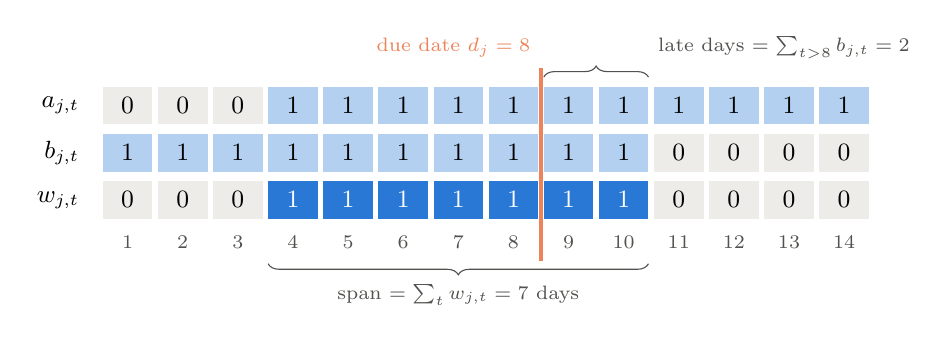
\begin{tikzpicture}[x=7mm,y=6mm,font=\small]
  \foreach \t in {1,...,14} { \node[cink,font=\scriptsize] at (\t,-0.9) {\t}; }
  \node[anchor=east] at (0.3,2) {$a_{j,t}$};
  \node[anchor=east] at (0.3,1) {$b_{j,t}$};
  \node[anchor=east] at (0.3,0) {$w_{j,t}$};
  \foreach \t in {1,...,14} {
    \pgfmathtruncatemacro{\A}{\t>=4 ? 1 : 0}
    \pgfmathtruncatemacro{\B}{\t<=10 ? 1 : 0}
    \pgfmathtruncatemacro{\W}{\A*\B}
    \ifnum\A=1 \def\ca{cblue!35}\else \def\ca{cgrey!60}\fi
    \ifnum\B=1 \def\cb{cblue!35}\else \def\cb{cgrey!60}\fi
    \ifnum\W=1 \def\cw{cblue}\def\tw{white}\else \def\cw{cgrey!60}\def\tw{black}\fi
    \fill[\ca] (\t-0.45,1.6) rectangle (\t+0.45,2.4);
    \node at (\t,2) {\A};
    \fill[\cb] (\t-0.45,0.6) rectangle (\t+0.45,1.4);
    \node at (\t,1) {\B};
    \fill[\cw] (\t-0.45,-0.4) rectangle (\t+0.45,0.4);
    \node[\tw] at (\t,0) {\W};
  }
  \draw[clate, line width=1.2pt] (8.5,-1.3) -- (8.5,2.8) node[above left, font=\scriptsize, text=clate] {due date $d_j=8$};
  \draw[decorate,decoration={brace,amplitude=4pt,mirror},cink] (3.55,-1.35) -- (10.45,-1.35)
     node[midway,below=4pt,font=\scriptsize] {span $=\sum_t w_{j,t}=7$ days};
  \draw[decorate,decoration={brace,amplitude=4pt},cink] (8.55,2.6) -- (10.45,2.6)
     node[pos=1,above right=3pt and 0pt,font=\scriptsize] {late days $=\sum_{t>8} b_{j,t}=2$};
\end{tikzpicture}
\caption{Time-window encoding for one project. $a$ switches on once and stays on, $b$ switches off
once and stays off, and $w=a\wedge b$ is the window. Span, late days and the late flag are linear
in these booleans, with no big-$M$ constant.}
\label{fig:window}
\end{figure}

From the window we read three quantities, all linear (\cref{fig:window}):
\begin{equation}
\mathrm{span}_j=\sum_{t\in\Hor} w_{j,t},\qquad
L_j=\sum_{t>d_j} b_{j,t},\qquad
\ell_j = b_{j,d_j+1}\ \ (\text{project late}),\qquad \text{for } d_j<h .
\label{eq:derived}
\end{equation}

\begin{proposition}[the window measures the schedule]\label{prop:window}
Let $x$ satisfy \eqref{c:day}--\eqref{c:cover} and let project $j$ be delivered with first and last
working days $s_j\le e_j$. (i) For every window $(a,b,w)$ compatible with $x$,
$\mathrm{span}_j\ge e_j-s_j+1$, $L_j\ge \max(0,e_j-d_j)$ and $\ell_j\ge[e_j>d_j]$. (ii) The
\emph{tight} window $a_{j,t}=[t\ge s_j]$, $b_{j,t}=[t\le e_j]$ satisfies
\eqref{c:mono}--\eqref{c:wy} and attains all three bounds with equality.
\end{proposition}
\begin{proof}
(i) By \eqref{c:inside}, $w_{j,s_j}=w_{j,e_j}=1$. By \eqref{c:mono} $a$ is non-decreasing and $b$
non-increasing, so $a_{j,t}=b_{j,t}=1$ for all $s_j\le t\le e_j$, hence $w_{j,t}=1$ there by
\eqref{c:and}; this gives the span bound. Since $b_{j,e_j}=1$ and $b$ is non-increasing,
$b_{j,t}=1$ for all $d_j<t\le e_j$, which gives the bounds on $L_j$ and $\ell_j$.
(ii) Direct substitution.
\end{proof}

So the model can \emph{overstate} a duration or a lateness but never understate it, and the true
value is always available to it. \Cref{sec:objectives} shows why this is enough.

\paragraph{Valid inequalities (cuts).}
They remove no schedule but help the solver prove optimality.
\begin{align}
\sum_{j\in\J} \Big(\sum_{k\in T\cap\QJ{j}} n_{j,k}\Big)\, y_j &\le \sum_{i:\ \QS{i}\cap T\neq\emptyset} \avail{i}
  && \forall\, T\subseteq \Q \quad\text{(Hall cuts)} \label{c:hall}\\
\mathrm{span}_j &\ge \max_{k\in\QJ{j}} \left\lceil \frac{n_{j,k}}{|\Sset_k|}\right\rceil y_j
  && \forall j\in\J \quad\text{(minimum span)} \label{c:span}
\end{align}
\eqref{c:hall} holds because every employee-day serves at most one unit of demand, and only
employees who hold a skill of $T$ can serve demand in $T$. \eqref{c:span} holds because at most
$|\Sset_k|$ people can work on skill $k$ in one day. In the code, \eqref{c:hall} is generated for
every subset $T$ (all $2^{10}-1$ subsets on medium and large) and kept only when it is not
trivially satisfied.

%=====================================================================
\section{Objectives}\label{sec:objectives}
%=====================================================================

\begin{table}[ht]
\centering\small
\renewcommand{\arraystretch}{1.25}
\begin{tabularx}{\linewidth}{@{}l l c X@{}}
\toprule
& \textbf{Objective} & \textbf{Sense} & \textbf{Linking constraints} \\
\midrule
$f_1$ & profit & max & $v_1 = \sum_j g_j y_j - \sum_j c_j L_j$ \\
$f_2$ & longest project span & min & $v_2 \ge \mathrm{span}_j\quad\forall j$ \\
$f_3$ & most projects per employee & min & $u_{i,j}\ge x_{i,j,k,t}$;\quad $v_3\ge\sum_j u_{i,j}\quad\forall i$ \\
$f_4$ & number of late projects & min & $v_4 = \sum_{j:\,d_j<h} \ell_j$ \\
$E_1$ & largest team on a project & min & $v_5\ge\sum_i u_{i,j}\quad\forall j$ \\
$E_2$ & utilisation gap (fairness) & min &
  $\rho_i=\big\lfloor 100\sum x_{i,\cdot,\cdot,\cdot}/\avail{i}\big\rfloor$;\ \ $\overline\rho\ge\rho_i$,\ $\underline\rho\le\rho_i$;\ \ $v_6=\overline\rho-\underline\rho$ \\
\bottomrule
\end{tabularx}
\caption{The six objectives. $f_1$--$f_4$ come from the brief; $E_1$ and $E_2$ are our additions.
$E_2$ is computed over employees who hold at least one needed skill and are not on leave for the
whole horizon, in \% of \emph{available} days so that holidays do not count as idleness.}
\label{tab:objectives}
\end{table}

\paragraph{Interpretation choices.} The brief leaves several points open; we chose what a real
company would do.
\begin{itemize}
  \item \emph{Execution time} is the calendar span of a project, holiday gaps included (the wait the
        client sees), and we minimise the \emph{longest} one.
  \item \emph{Projects per employee} is minimised for the \emph{most loaded} employee: one overloaded
        person is what hurts.
  \item Only \emph{delivered} projects can be late; a rejected project is declined, not late.
  \item $E_1$ measures coordination cost (meetings, hand-overs). $E_2$ measures fairness.
\end{itemize}

\paragraph{One-sided linking is exact.} For the minimised objectives, $v$ is only bounded from
below, and $f_1$ is an equality over $L_j$, which is itself only bounded from below. Write every
objective as a minimisation, $\tilde f=(-f_1,f_2,\dots)$, and let $F(x)$ be the true values of a
schedule $x$ (as recomputed by the independent checker).

\begin{proposition}\label{prop:onesided}
(i) Every feasible solution satisfies $\tilde v\ge F(x)$ componentwise. (ii) For every feasible $x$
there is a completion with $\tilde v=F(x)$. Consequently, (iii) minimising a weighted sum
$\sum_k\lambda_k\tilde v_k$ with all $\lambda_k>0$ returns $\tilde v=F(x)$ at the optimum, and (iv)
adding a constraint of the form $\tilde v_k\le\varepsilon$ removes exactly the schedules with
$F_k(x)>\varepsilon$, and no others.
\end{proposition}
\begin{proof}
(i) and (ii) follow from \cref{prop:window} and from $u$, $\overline\rho$, $\underline\rho$ being
only bounded from the side that makes $v$ an over-estimate. (iii) If some $\tilde v_k>F_k(x)$, the
tight completion of (ii) is feasible and has a strictly smaller weighted sum. (iv) If
$F_k(x)\le\varepsilon$, the tight completion satisfies the new constraint; if $F_k(x)>\varepsilon$,
then $\tilde v_k\ge F_k(x)>\varepsilon$ for every completion.
\end{proof}

A non-optimised objective may still come back overstated, which is why we never report solver values:
every schedule is re-evaluated by the checker.

%=====================================================================
\section{Computing the Pareto front}
%=====================================================================

\begin{definition}
Plan $x$ \emph{dominates} plan $x'$ if $F(x)\le F(x')$ componentwise (all objectives written as
minimisations) with at least one strict inequality. $x$ is \emph{Pareto-optimal} if no plan dominates
it; its image $F(x)$ is a \emph{non-dominated point}. The \emph{front} is the set of non-dominated
points.
\end{definition}

All objectives are integers with known bounds $[\mathrm{lb}_k,\mathrm{ub}_k]$, so the front is finite.
Both methods below solve a \emph{profit-first weighted sum}
\begin{equation}
\min\ \; -R\,v_1+\sum_{k\ge2} v_k, \qquad R = 1+\sum_{k\ge 2}(\mathrm{ub}_k-\mathrm{lb}_k).
\label{eq:weighted}
\end{equation}
One unit of profit outweighs any change in all other objectives together, and every weight is
strictly positive.

\begin{lemma}\label{lem:ws}
An optimal solution of \eqref{eq:weighted}, under any additional constraints of the form used below,
is Pareto-optimal among the plans that satisfy those constraints.
\end{lemma}
\begin{proof}
A plan that dominates it and satisfies the same constraints would have a strictly smaller weighted
sum, because all weights are positive (and by \cref{prop:onesided}(iii) the optimum is evaluated at
its true values).
\end{proof}

\subsection{\texorpdfstring{$\varepsilon$}{Epsilon}-constraint (two objectives)}

\begin{algorithm}[H]
\caption{$\varepsilon$-constraint for (profit, $f$)}\label{alg:eps}
\begin{algorithmic}[1]
\State $\varepsilon\gets\mathrm{ub}_f$, \ $P\gets\emptyset$
\Loop
  \State solve \eqref{eq:weighted} over (profit, $f$) subject to $v_f\le\varepsilon$
  \If{infeasible} \Return $P$ \EndIf
  \State $p\gets F(\text{solution})$ \Comment{true values, from the checker}
  \State $P\gets P\cup\{p\}$; \ $\varepsilon\gets p_f-1$
  \If{$p_f=\mathrm{lb}_f$} \Return $P$ \EndIf
\EndLoop
\end{algorithmic}
\end{algorithm}

The tie-breaking term $+v_f$ in \eqref{eq:weighted} prevents weakly dominated points. Each iteration
lowers $\varepsilon$ by at least one, so at most $\mathrm{ub}_f-\mathrm{lb}_f+1$ solves are needed.

\subsection{Disjunctive exclusion (any number of objectives)}

\begin{algorithm}[H]
\caption{Disjunctive exclusion}\label{alg:disj}
\begin{algorithmic}[1]
\State $P\gets\emptyset$
\Loop
  \State solve \eqref{eq:weighted} subject to all exclusion constraints added so far
  \If{infeasible} \Return $P$ \EndIf
  \State $p\gets F(\text{solution})$; \ $P\gets P\cup\{p\}$
  \State add booleans $\lambda_1,\dots,\lambda_K$ with $\lambda_k \Rightarrow \tilde v_k\le \tilde p_k-1$
  \State add $\sum_k\lambda_k\ge1$ \Comment{beat $p$ strictly on some objective}
\EndLoop
\end{algorithmic}
\end{algorithm}

\begin{theorem}[exactness]\label{thm:exact}
If every solve in \cref{alg:disj} is proven optimal, the returned set $P$ is exactly the front.
\end{theorem}
\begin{proof}
\emph{No false point.} Let $p$ be found after points $p^1,\dots,p^r$. Suppose a plan $q$ dominates
$p$. Since $p$ beats each $p^s$ strictly on some objective and $q$ is at least as good as $p$
everywhere, $q$ also beats each $p^s$ on that objective, so $q$ satisfies every exclusion and has a
strictly smaller weighted sum (\cref{lem:ws}): a contradiction with the optimality of $p$.
\emph{No missing point.} Let $q$ be a non-dominated point not in $P$. For every $p\in P$, $p$ does
not dominate $q$ and $p\neq q$, so $q$ is strictly better than $p$ on some objective. Hence a plan
with image $q$ satisfies every exclusion (\cref{prop:onesided}(iv)), and the last model was not
infeasible: a contradiction.
\emph{Termination.} Each found point is excluded and the objective space is a finite integer box.
\end{proof}

\begin{remark}[time limits]
With a time limit, a solve may return a good but unproven plan $p$. The exclusion added after $p$
still never removes a non-dominated point (same argument as ``no missing point''), so the search
stays safe; only the guarantee that each \emph{found} point is Pareto-optimal is lost. The notebook
therefore marks each point as \texttt{proven} (its solve was optimal, so it is Pareto-optimal) or
not, and reports \texttt{exact = True} only when every solve was proven and the last model was
infeasible. Each solve is warm-started from the previous point's schedule, which changes speed
only.
\end{remark}

%=====================================================================
\section{A solver-independent certificate for the maximum profit}
%=====================================================================

CP-SAT reports \texttt{OPTIMAL} for the maximum profit, but a certificate that can be checked step by
step is stronger. It rests on a classical result.

\begin{theorem}[Hall / Gale]\label{thm:hall}
Ignoring due dates, a set $P\subseteq\J$ of projects can be fully staffed if and only if
\[
\sum_{j\in P}\ \sum_{k\in T\cap\QJ{j}} n_{j,k} \;\le \sum_{i:\ \QS{i}\cap T\neq\emptyset}\avail{i}
\qquad\forall\, T\subseteq\Q .
\]
\end{theorem}
\begin{proof}[Sketch]
Build a bipartite flow network: each employee-day $(i,t)$, $t\notin\V{i}$, has supply $1$ and is
linked to the skills in $\QS{i}$; each skill $k$ has demand $D_k=\sum_{j\in P}n_{j,k}$. Since all
demand units of one skill are interchangeable, $P$ is staffable iff this transportation problem is
feasible, and by max-flow/min-cut (Gale's theorem) this holds iff $D(T)\le|N(T)|$ for every set of
skills $T$, which is the stated inequality.
\end{proof}

\noindent The certificate has three steps.
\begin{enumerate}
  \item \textbf{Bound.} Penalties are non-negative, so a plan delivering exactly $P$ earns at most
        $g(P)=\sum_{j\in P}g_j$.
  \item \textbf{Enumerate.} Given the best profit found $z$, a depth-first search with the bound
        ``gain so far + gain of all remaining projects $\le z$ $\Rightarrow$ prune'' lists every
        set $P$ that passes all Hall inequalities and has $g(P)>z$. By \cref{thm:hall}, no other set
        can beat $z$.
  \item \textbf{Rule out.} For each listed $P$, a small CP-SAT model (only the projects of $P$)
        asks: can $P$ be staffed with total lateness penalty $\le g(P)-z-1$? \texttt{INFEASIBLE}
        means $P$ cannot beat $z$. If a plan is found, $z$ increases and the search continues.
\end{enumerate}
When every listed set is ruled out, $z$ is the maximum profit. The final plan is re-checked by the
independent checker.

%=====================================================================
\section{Results}\label{sec:results}
%=====================================================================

All numbers come from one full run of the notebook (OR-Tools CP-SAT, 14 threads, about 16 minutes).
Medium and large Pareto fronts are time-limited (10\,s per solve, 2--6\,min per front), so their
exact counts can shift slightly between runs; every other number is exact.

\subsection{The instances}

\begin{table}[H]
\centering\small
\begin{tabular}{@{}lrrrrr@{}}
\toprule
Instance & days $h$ & employees & projects & $x$-variables & demand / capacity \\
\midrule
toy    & 5  & 3 & 5  & 90    & 1.08 \\
medium & 22 & 5 & 15 & 1{,}298 & 1.32 \\
large  & 36 & 6 & 25 & 3{,}939 & 1.41 \\
\bottomrule
\end{tabular}
\caption{The three given instances. All ask for more person-days than the staff can supply.}
\end{table}

\begin{figure}[H]
\centering
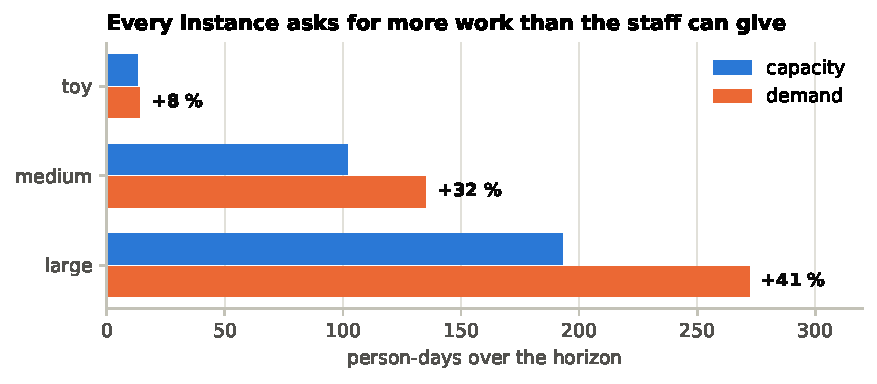
\includegraphics[width=0.92\linewidth]{figures/demand_vs_capacity.pdf}
\caption{Total demand against total capacity. No single skill is overbooked, but the same people
hold several skills, so the projects compete for them: some must be declined.}
\end{figure}

\subsection{Maximum profit, certified}

\begin{table}[H]
\centering\small
\begin{tabular}{@{}lrrr@{}}
\toprule
& toy & medium & large \\
\midrule
Maximum profit (CP-SAT, 30\,s, \texttt{OPTIMAL}) & 65 & 413 & 817 \\
Sum of all gains (trivial bound) & 80 & 510 & 1{,}020 \\
Hall bound (best staffable project set) & 70 & 440 & 860 \\
Candidate sets that could beat the best plan & 1 & 38 & 775 \\
Sub-models solved / unresolved & 4 / 0 & 76 / 0 & 1{,}550 / 0 \\
Certificate time & $<0.1$\,s & 3.1\,s & 95.6\,s \\
Late projects in the maximum-profit plan & 0 & 3 & 2 \\
\bottomrule
\end{tabular}
\caption{The certificate of \cref{thm:hall} proves all three maxima independently of CP-SAT's own
optimality proof. Being late on a lucrative project can be worth more than declining it.}
\end{table}

\begin{figure}[H]
\centering
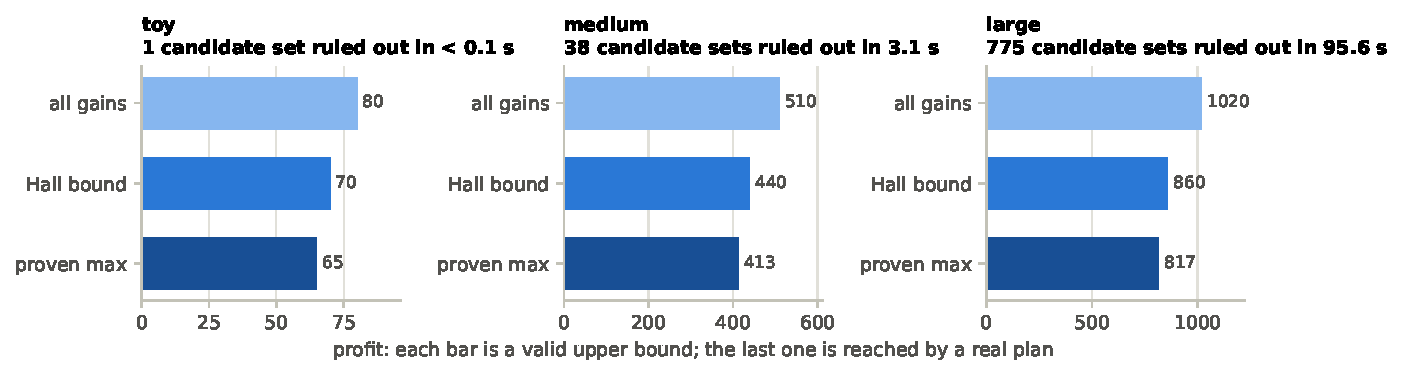
\includegraphics[width=\linewidth]{figures/proof_ladder.pdf}
\caption{Proof ladder: each bar is a valid upper bound on the profit, and the last one is reached by
a real plan.}
\end{figure}

\subsection{Toy instance: exact fronts}

The two methods return identical fronts for profit against each of the five other objectives, all
proven exact. With the brief's four objectives, \cref{alg:disj} finds 13 Pareto-optimal plans
(\cref{tab:toy}); with all six objectives, 18.

\begin{table}[H]
\centering\small
\begin{tabular}{@{}rrrr|rrrr@{}}
\toprule
profit & longest & proj./emp. & late & profit & longest & proj./emp. & late \\
\midrule
65 & 2 & 3 & 0 & 40 & 3 & 1 & 0 \\
65 & 3 & 2 & 0 & 37 & 1 & 2 & 1 \\
59 & 1 & 4 & 1 & 35 & 1 & 2 & 0 \\
55 & 2 & 2 & 0 & 30 & 2 & 1 & 0 \\
49 & 1 & 3 & 1 & 20 & 1 & 1 & 0 \\
45 & 1 & 3 & 0 & 0 & 0 & 0 & 0 \\
42 & 3 & 1 & 1 & & & & \\
\bottomrule
\end{tabular}
\caption{The exact front of the toy instance for the brief's four objectives (13 plans). The empty
plan is always Pareto-optimal, because every minimised objective improves by doing nothing.}
\label{tab:toy}
\end{table}

\begin{figure}[H]
\centering
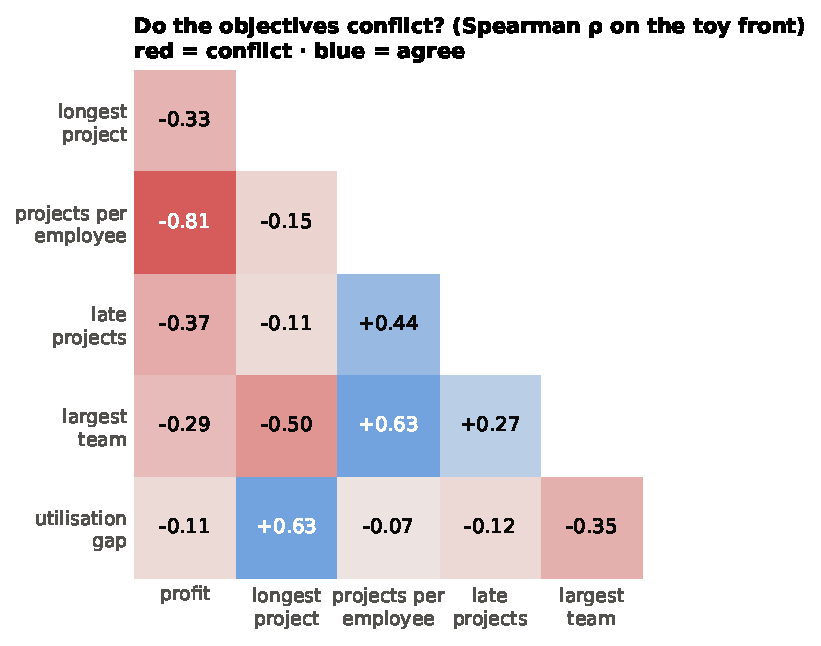
\includegraphics[width=0.7\linewidth]{figures/conflict_heatmap.pdf}
\caption{Spearman correlation between objectives on the exact six-objective front (all oriented
``smaller is better''; negative = conflict). Profit conflicts most with focus ($-0.81$); small
teams make projects longer ($-0.50$); fairness barely costs profit ($-0.11$).}
\end{figure}

\subsection{Medium and large: trade-offs under a time budget}

On medium, the four-objective search ran for 6 minutes and found 30 mutually non-dominated plans, 2
of them proven Pareto-optimal. On large, we computed profit against each other objective, 2 minutes
per pair.

\begin{figure}[H]
\centering
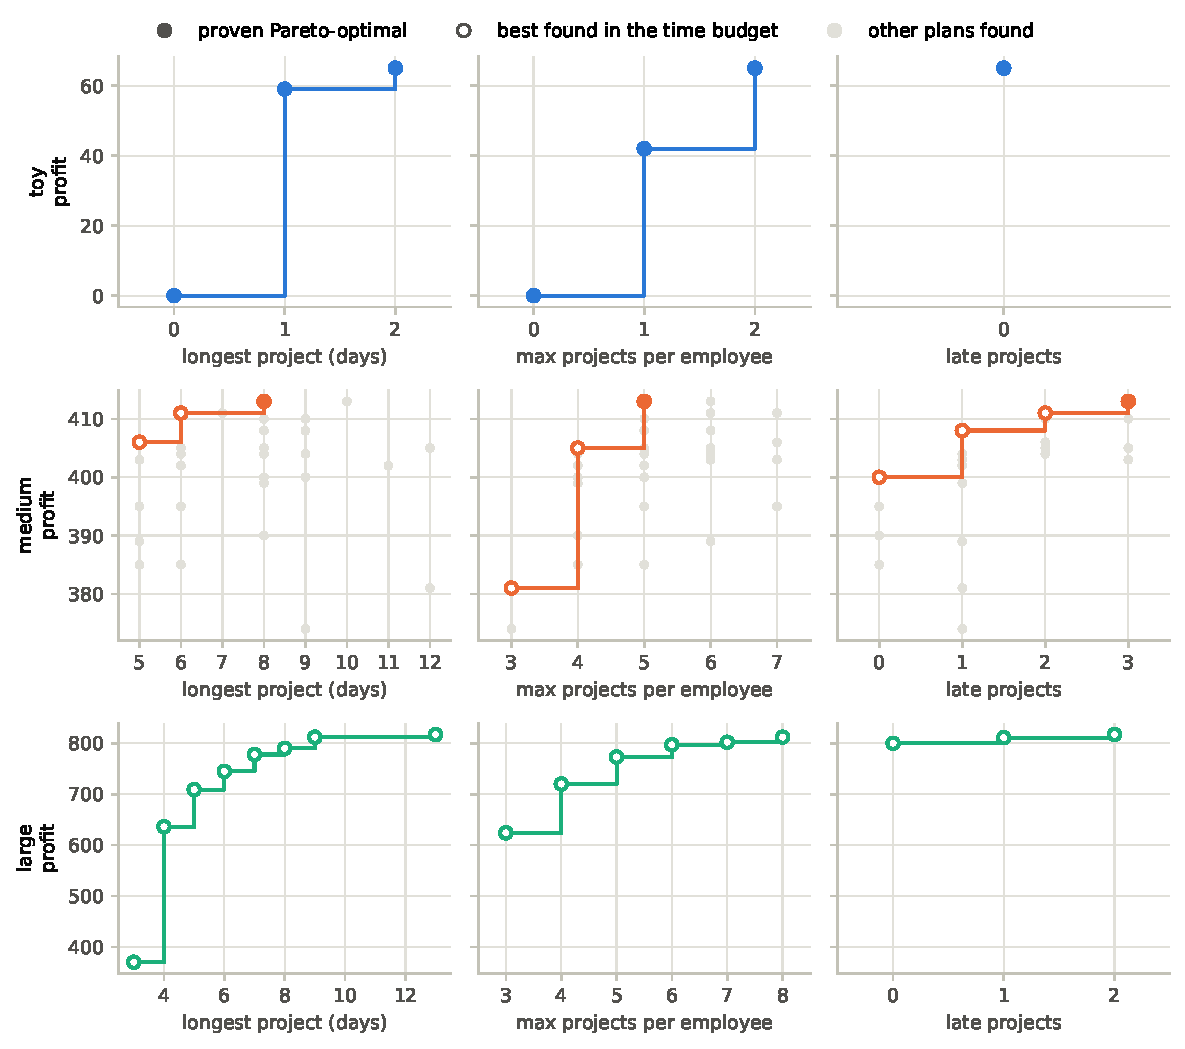
\includegraphics[width=\linewidth]{figures/fronts_brief.pdf}
\caption{Profit against each brief objective. The staircase links the plans that are non-dominated
in that two-objective view; filled = proven Pareto-optimal, hollow = best found in the budget, grey
= other plans found.}
\end{figure}

\begin{table}[H]
\centering\small
\begin{tabular}{@{}lcc@{}}
\toprule
Best plan for\ldots\ (profit $\ge 70\,\%$ of max) & medium & large \\
\midrule
fewest late projects & 0 late, profit 400 ($-3.1\,\%$) & 0 late, profit 800 ($-2.1\,\%$) \\
shortest longest project & 5 days, profit 406 ($-1.7\,\%$) & 4 days, profit 636 ($-22.2\,\%$) \\
fewest projects per employee & 3, profit 381 ($-7.7\,\%$) & 3, profit 624 ($-23.6\,\%$) \\
fairest (utilisation gap) & -- & gap 0, profit 733 ($-10.3\,\%$)$^{*}$ \\
\bottomrule
\end{tabular}
\caption{The price of each objective, relative to the certified maximum profit.
$^{*}$Least stable pair: with 2 minutes, the best fully fair plan found ranged from 628 to 800 across
our runs.}
\label{tab:price}
\end{table}

\begin{figure}[H]
\centering
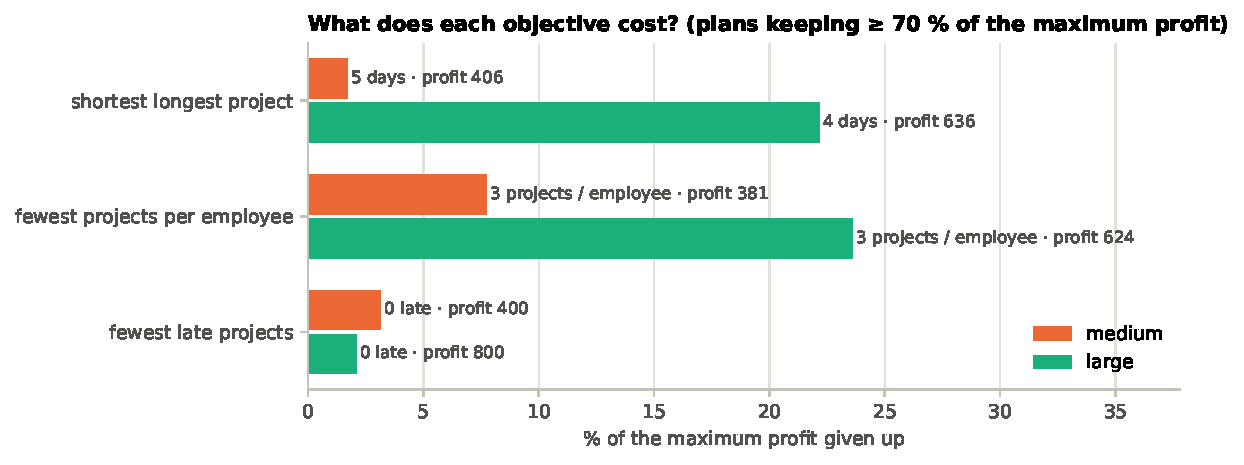
\includegraphics[width=\linewidth]{figures/price_of_objectives.pdf}
\caption{The same information as \cref{tab:price}: punctuality is cheap on both instances; focused
employees are expensive, and short projects are expensive on large.}
\end{figure}

\begin{sidewaysfigure}
\centering
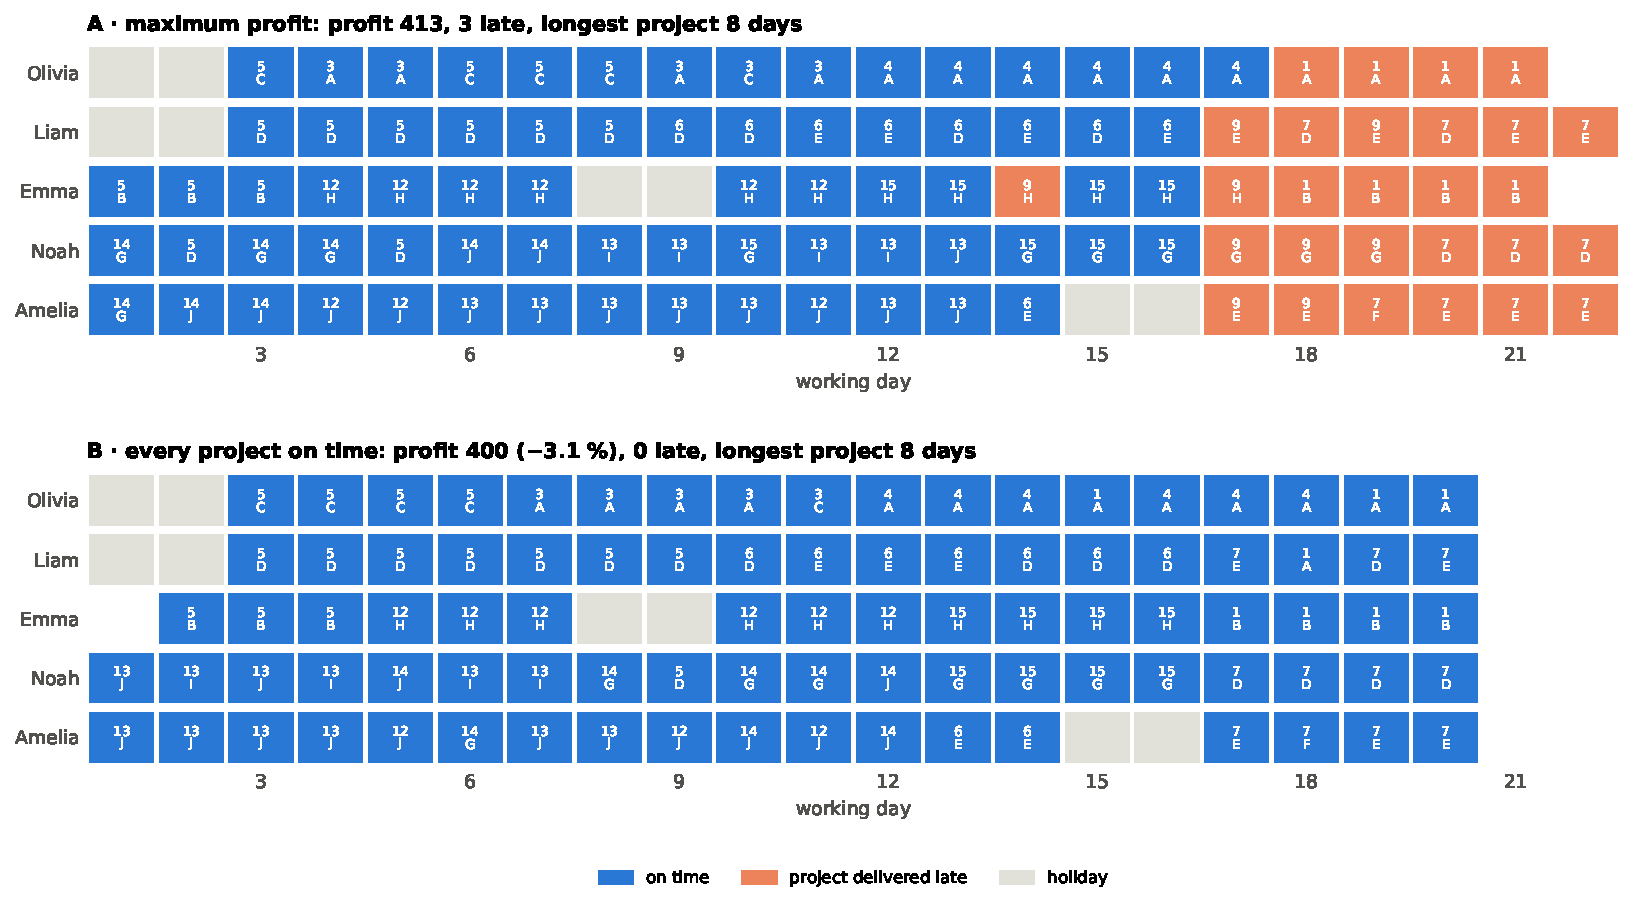
\includegraphics[width=\linewidth]{figures/schedule_medium_tradeoff.pdf}
\caption{Decision space on medium. Rows are employees, columns are days, each cell is
\emph{project / skill}. Plan A earns the maximum but delivers 3 projects late (orange); plan B
gives up 3.1\,\% and delivers everything on time.}
\label{fig:gantt}
\end{sidewaysfigure}

\subsection{Verification and scaling}

\begin{itemize}
  \item \textbf{Brute force.} On 10 random tiny instances (3 days, 2 employees, 3 projects), we list
        every possible schedule, keep the feasible ones, filter the non-dominated ones and compare
        them with the solver's front, for 4 and for 6 objectives: identical in \textbf{20 / 20}
        cases.
  \item \textbf{Two methods.} $\varepsilon$-constraint and disjunctive exclusion agree on every
        two-objective toy front.
  \item \textbf{Independent checker.} Every reported plan re-passes rules R1--R5, and every
        objective is recomputed from the raw assignments.
  \item \textbf{Scaling.} On generated instances, the exact (profit, longest project) fronts are all
        proven, in under 10\,s up to about 1{,}350 decision variables, but the time grows quickly
        and unevenly with size.
\end{itemize}

%=====================================================================
\section{Limitations and next steps}
%=====================================================================

\begin{itemize}
  \item \textbf{Proving is the bottleneck, not finding.} Good plans appear within seconds; proving
        that no better plan exists takes hours on medium and large with three or more objectives.
        Those fronts are valid, mutually non-dominated plans with the proven points marked.
  \item \textbf{A faster exact method} would decompose the problem: choose the project set first (a
        knapsack with Hall constraints, as in the certificate), then schedule it. The certificate
        shows this works for one objective.
  \item \textbf{Interpretation.} Other readings of the brief (total instead of maximum duration,
        total employee--project pairs instead of the most loaded employee) change the front. Each is
        a one-line change of the linking constraints in \cref{tab:objectives}.
  \item \textbf{The generator} is calibrated on the three given files only (gain grows with workload
        and urgency, one holiday block per employee).
\end{itemize}

\appendix
%=====================================================================
\section{Comparison with the course reference model}
%=====================================================================

The reference model (notation, decision variables and full MILP) is reproduced in the repository
folder \texttt{02\_reference\_model/}.

\begin{table}[H]
\centering\small
\renewcommand{\arraystretch}{1.2}
\begin{tabularx}{\linewidth}{@{}l X X@{}}
\toprule
& \textbf{Reference MILP (course)} & \textbf{This project (CP-SAT)} \\
\midrule
Assignment & $X_{i,j,k,t}$ for every $i,j,k,t$; illegal ones fixed to $0$ & $x$ created only on legal slots $\Leg$ \\
Coverage & $n_{j,k}Y_j\le\sum X\le n_{j,k}$ & $\sum x=n_{j,k}y_j$ (no useless work) \\
End date & $E_j\ge t\,X_{i,j,k,t}$ & window $b_{j,t}$ (also gives the start, hence the span) \\
Lateness & $L_j\ge E_j-d_j$ & $L_j=\sum_{t>d_j}b_{j,t}$ \\
Objectives & profit only & profit + 3 brief objectives + 2 of ours \\
Solver & Gurobi (licence) & OR-Tools CP-SAT (free, parallel, proves optimality) \\
Output & one optimal plan & the full non-dominated set + a certificate for the maximum profit \\
\bottomrule
\end{tabularx}
\caption{Both models have the same maximum profit on every instance; ours adds the measurements
needed by the other objectives and removes partial work on rejected projects.}
\end{table}

\end{document}
